%----------------------------------------------------------------------------------------
%	PART III
%----------------------------------------------------------------------------------------

\part{Nyxi Sciences}

%----------------------------------------------------------------------------------------
%	Tenebrivity
%----------------------------------------------------------------------------------------

\chapterimage{placeholder.png} % Chapter heading image

\chapter{Tenebrivity}

One of the most significant impacts that the Nyxi had on human civilization was
a full understanding of what we used to call dark matter. At the time, in spite
of hundreds of years of research, humanity was still unable to make any
progress understanding dark matter beyond theoretical pursuits, especially
since we lacked any significantly accessible dark matter to attempt more
advanced measurements or any experiments. Meanwhile, we learned that the
Nyxophora is abundant with dark matter, to the extent that it's even used in
the biochemistry of the Nyxi. After first contact and overcoming the
difficulties of communication, one of the first provisions from the Nyxi was a
full explanation of dark matter, which is now referred to as tenebrum, and an
abundance of access to it. While it took quite some time to understand their
theory in the context of humanity's framework of physics, the final result -
the Theory of Tenebrivity - revolutionized our understanding of the universe
and our technological capabilities.

The complete theory is organized hierarchically by scale, extending all of our
prior models of the universe. From the smallest to largest scales, the theory's
components are described by:
\begin{description}
  \item[Fractolet-T Theory] The extension of Fractolet Theory, the current most
    fundamental Theory of Everything, extended to include additional
    semidimensional stabilian and diffusian fractolets that interact to create
    umbristrings and tenebranes.
  \item[Tenebrivic Fractobrane-String Theory] The theory that describes how
    umbristrings and tenebranes resonate and interact to form the quantum
    tenebrivic particle fields.
  \item[Quantum Tenebridyanmics] The quantum field theory of tenebrivic particles. This
    theory explains the fundamental tenebrivic force, the composite particles
    formed from confinement, and the fundamental model of atomoxes - atom-like
    structures formed by tenebrivic particles.
  \item[Tenebrichemistry] The full theory of how differing atomoxes form the
    netherelements, which in turn form the nethermolecules, and the resulting
    chemical interactions.
  \item[Tenebrum Dynamics] The human-scale study of tenebrum and its properties,
    especially in relation to the mechanics of lux matter.
  \item[Tenebrivic Cosmology] The impact that tenebrum has had on the structure and
    evolution of the universe.
\end{description}

A deep treatise of the two smallest-scale theories are well beyond the scope of
this book and require an extensive background in theoretical physics, but we'll
briefly review the concepts included. Beyond that, we'll then go into the
essential formalism of each theory which will serve as an effective
introduction if you wish to dive deeper into the relevant branch of science.

\section{Fractolets, Umbristrings, Tenebranes}

\section{Quantum Tenebridynamics}

Quantum Tenebridynamics (QTD) is the theory that describes tenebrivity, one of
the five known fundamental forces of nature. This force binds dark matter
particles to create the fundamental structures of the atomox. Unlike the
electromagnetic force where particles have an electric charge (positive,
negative), in QTD, particles carry a "tenebridge". There are four tenebridgials
- types of tenebridge - which are named after the four luminous classical
elements in Nyx antiquity:
\begin{center}vortex, crystal, flow, and spark\end{center}
There is also the concept of have a negative tenebridge values, labelled by the antitenebridgials:
\begin{center}antivortex, anticrystal, antiflow, and antispark\end{center}
Keep in mind that these terms are simply labels, and otherwise not at all related to vortices, crystals, flows, or sparks.

QTD involves four total particles: two dark fermions (matter particles), and
two gauge bosons (force carriers).
\begin{table}[h]
  \centering
  \begin{tabular}{c c c c c l}
    \toprule
    \textbf{Particle}                         & \textbf{Field}          & \textbf{Type} & \textbf{Spin}     & \textbf{Mass}              & \textbf{Kinetic Term} \\
    \midrule
    \textbf{Xenobron}                         & $X$                     & boson         & 1                 & 0                          & \(
    -\frac{1}{4}\Xi_{\mu \nu}\Xi^{\mu \nu}
    \)                                                                                                                                                           \\
    \\
    \textbf{Noxion}                           & $\xi^{\sigma}_{\alpha}$ & fermion       & 1/2               & 0                          & \(
    +i \delta_{\sigma \tau} \bar{\xi}^{\alpha}_{\sigma} \gamma^{\mu}_{\alpha \beta} \partial_{\mu} \xi^{\beta}_{\tau} \)                                         \\ \\ \textbf{Vanibron}       &
    $V_{\alpha\bar{\beta}}$                   & boson                   & 1             & 0                 & \( -\frac{1}{4}\Theta_{\mu
    \nu}\Theta^{\mu \nu} \)                                                                                                                                      \\ \\ \textbf{Thuleon}                          &
    $\eth^{\sigma}_{\alpha\bar{\beta}\gamma}$ & fermion                 & 3/2           & $m_{t}$, $-m_{t}$ &
       \( +\Upsilon_{\omega} \left[
         -\frac{i}{2}\bar{\Theta}_{\mu}\gamma^{\mu\nu\rho}\nabla_{\mu}\Theta_{\rho}
    \right]^{\omega} \)                                                                                                                                          \\  &  &  &  &  & -\bar{\Theta}_{\mu}M^{\mu\nu}\Theta_{\nu}
    \bottomrule
  \end{tabular}
  \caption{Summary of Particles in QTD}
\end{table}

Interactions

\begin{table}[h]
  \centering
  \begin{tabular}{c c c c c c}
    \toprule
    \textbf{Interaction} & \textbf{Diagram}     & \textbf{Conservation} & \textbf{Formula}                                        \\
    \midrule
    \textbf{nox-xen-nox} & \qtdint[0.1]{bw-nxn} & \qtdint[0.1]{cl-nxn}  & \(n_i + \bar{n}_{\bar{i}} \rightarrow x\)               \\
                         &                                                                                                        \\
    \textbf{nox-van-nox} & \qtdint[0.1]{bw-nvn} & \qtdint[0.1]{cl-nvn}  & \(n_i + \bar{n}_{\bar{j}} \rightarrow v_{i\bar{j}} \)   \\
                         &                                                                                                        \\
    \textbf{van-xen-van} & \qtdint[0.1]{bw-vxv} & \qtdint[0.1]{cl-vxv}  & $v_{i\bar{j}} + v_{j\bar{i}} \rightarrow x $            \\
                         &                                                                                                        \\
    \textbf{van3}        & \qtdint[0.1]{bw-v3}  & \qtdint[0.1]{cl-v3}   & $v_{i\bar{j}} + v_{k\bar{i}} \rightarrow v_{k\bar{j}} $ \\
    \bottomrule
  \end{tabular}
  \caption{Summary of Particles in QTD}
\end{table}

As we review each particle, we will also slowly build up the total Lagrangian
(\(\mathcal{L}_{\text{QTD}}\)) which encodes the dynamics of QTD.

\subsection{Noxion}
The noxion is the foundational particle of QTD, as it is the matter particle
that carries a single tenebridgial. Its antiparticle is the antinoxion, which
carries a single antitenebridgial. Since the noxions/antinoxions have no mass,
electric charge, color charge, or flavour, they have zero direct interaction
with any other fundamental force. This lack of interaction kept humanity from
coming to a viable understanding of dark matter at a distance.

\subsubsection{Diagram Representation}
Noxions are represented by an arrowed line in Feynman diagrams; for
antinoxions, this arrow faces left instead.

\hfill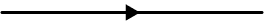
\includegraphics[width=0.5\textwidth]{tenebrivity/line-n.png}\hspace*{\fill}

\subsubsection{Quantum Field}
In order to properly represent the quantum noxion field, we have to account for
the noxion a spin-\(\frac{1}{2}\) Dirac spinor, as well as having tenebridge.
Therefore, the quantum noxion field can be written as:
\[
  \xi^{\sigma}_{\tau}
\]
where \(\sigma\) is an index (from 0 to 3) to represent the four spinor
components
\[
  \{ \text{spin-up noxion},\ \text{spin-down noxion},\ \text{spin-down antinoxion},\ \text{spin-up antinoxion} \},
\]
and \(\tau\) is an index (from 0 to 3) to represent the four tenebridgial
components
\[
  \{ \text{vortex noxion},\ \text{crystal noxion},\ \text{flow noxion},\ \text{spark noxion} \}.
\]

In summary, the quantum noxion field is a 16-component bispinor tenebridgial
field \(\xi^{\sigma}_{\tau}\)

\subsubsection{Lagrangian Contribution}

The motion of a free noxion particle contributes a kinetic term to the
Lagrangian:
\[
  \mathcal{L}_{\text{nox}} = i \delta_{\sigma \tau} \bar{\xi}^{\alpha}_{\sigma} \gamma^{\mu}_{\alpha \beta} \partial_{\mu} \xi^{\beta}_{\tau}
\]

\subsection{Xenobron}
The xenobron is a force carrier in QTD that is commonly involved in processes
of matter-antimatter annihilation, as well as enabling orbitals in atomoxes.
Xenobrons do not ever carry tenebridge, so their interaction with noxions is
exceptionally simple. In fact, since xenobrons are also spin-1 chargeless
massless bosons, they is only distinguishable from photons because they
interact with noxions while photons do not.

\subsubsection{Diagram Representation}
Xenobrons are represented by a dotted line, arrowless as the xenobron is its
own antiparticle

\hfill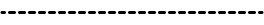
\includegraphics[width=0.5\textwidth]{tenebrivity/line-x.png}\hspace*{\fill}

\subsubsection{Quantum Field}

The quantum xenobron field is constructed as a \textit{spacetime} four-vector
field, written as:
\[
  X_{\mu}(\textbf{x})
\]
where \(\mu\) is an index (from 0 to 3) to represent the four dimensions of
spacetime
\[ \{t,\ x,\ y,\ z \} \].
One way to interpret this vector field is: for a given point in spacetime \(\textbf{x}\), \(X_{\mu}(\textbf{x})\) is the \(\mu\)-direction component of the quantum xenobron field.

\subsubsection{Lagrangian Contribution}

First we define the xenobronic field strength tensor \(\Xi\) to capture each
partial derivative of each component:
\[
  \Xi_{\mu \nu} = \partial_{\mu} X_{\nu} - \partial_{\nu} X_{\mu}.
\]
Then, the kinetic term of a free xenobron is described by:
\[
  \mathcal{L}_{\text{xen}} = -\frac{1}{4}\Xi_{\mu \nu}\Xi^{\mu \nu}
\]

\subsection{Noxion-Xenobron-Noxion Interaction}
Noxions can exhibit one type of interaction with other noxions mediated by the
xenobron; this interaction is sometimes called the nullary-component of
tenebrivity. Historically, the Nyxi first considered this interaction to be a
separate force from the other QTD interactions, as it's the only interaction
that acts at long distances. QTD was the theory that unified this interaction
with the rest.

\subsubsection{Diagram Representation}
The noxions and xenobrons interact via the noxion-xenbron-noxion (nxn)
interaction vertex:

\hfill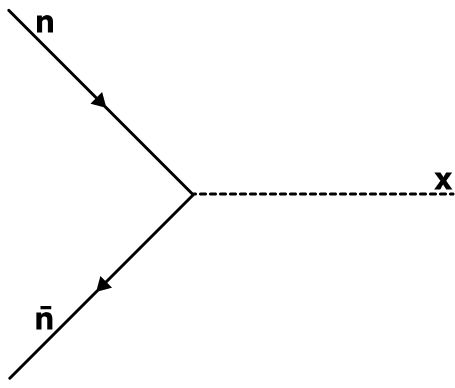
\includegraphics[width=0.35\textwidth]{tenebrivity/bw-nxn.png}\hspace*{\fill}

\subsubsection{Tenebridge Conservation}

Each vertex must conserve tenebridge, and therefore restricts which particles
and tenebridgials can be involved in the interaction. One simple way to analyze
this is by assigning a visual color to each tenebridgial, and looking at an
example of where the tenebridgials travel throughout the interaction. This
vertex is rather simple to analyze this way:

\hfill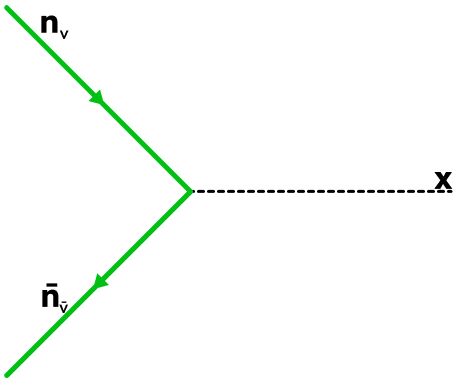
\includegraphics[width=0.35\textwidth]{tenebrivity/cl-nxn.png}\hspace*{\fill}

Thus we see tenebridge is conserved by following the noxion path. Therefore,
the fundamental restriction on this interaction is as follows:
\[
  n_{\alpha} + \bar{n}_{\bar{\alpha}} \rightarrow x
\]
Note that this equivalently describes the vertex \(n_{\alpha} \rightarrow
n_{\alpha} + x \) as all rotations of the diagram are valid as well.

\subsubsection{Lagrangian Contribution}
This vertex provides an interaction term for the Lagrangian:
\[
  \mathcal{L}_{\text{nxn}} = -c_{nxn} \delta_{ij} \bar{\xi}^{\alpha}_{i} \gamma^{\mu}_{\alpha \beta} \bar{\xi}^{\beta}_{j} X_{\mu}
\]
where \(c_{nxn}\) is the coupling constant that determines the strength of the
interaction.

\subsection{Vanibron}
\subsubsection{Diagram Representation}
\subsubsection{Quantum Field}
\subsubsection{Lagrangian Contribution}

\subsection{Noxion-Vanibron-Noxion}
\subsubsection{Diagram Representation}
\subsubsection{Tenebridge Conservation}
\subsubsection{Lagrangian Contribution}

\subsection{Vanibron-Xenobron-Vanibron}
\subsubsection{Diagram Representation}
\subsubsection{Tenebridge Conservation}
\subsubsection{Lagrangian Contribution}

\subsection{Vanibron-Xenobron-Vanibron}

\section{Nyxian Essences}

\begin{remark}
  In antiquity, the Nyxi defined eight different elements, influenced by the nature of their gaseous planet:
  \begin{description}
    \item[Active Elements] Flow, Spark, Vortex, and Crystal
    \item[Passive Elements] Hiatus, Mist, Lag, and Aurora
  \end{description}
\end{remark}